\chapter{Functional Requirements}
\section{Useage Model}
\scalebox{0.6}{
	
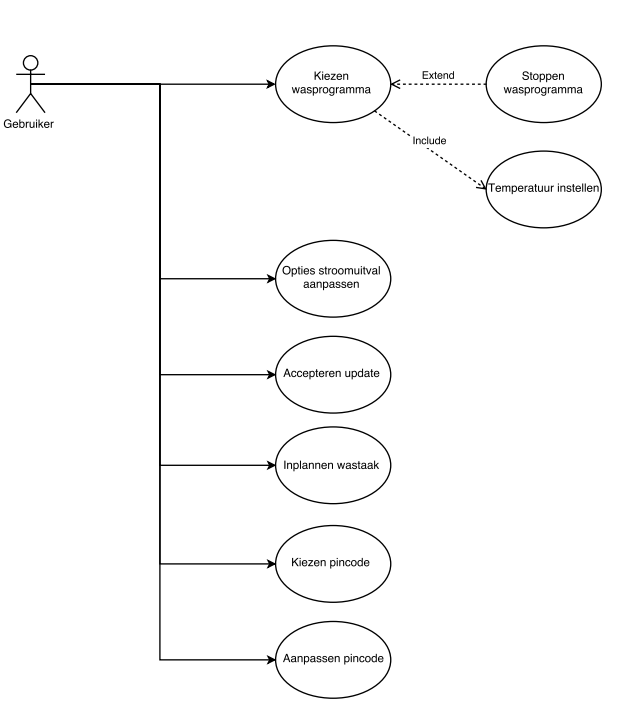
\includegraphics{usage_1.png}
}
\newpage
\scalebox{0.6}{
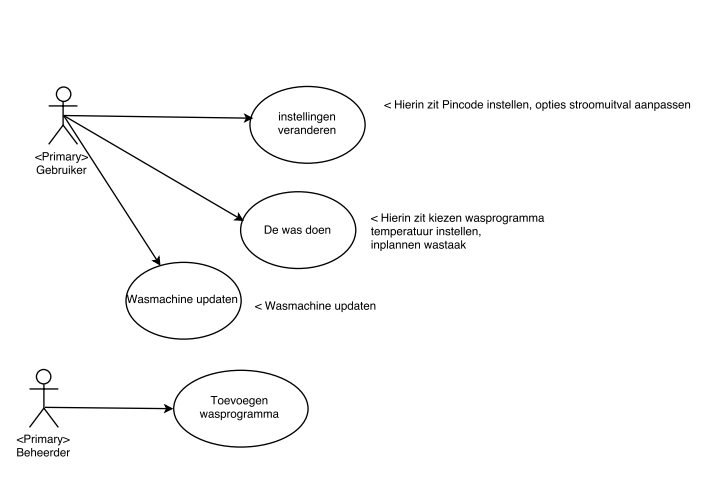
\includegraphics{usage_2.png}
	
}
\section{Inleiding}
In dit hoofdstuk zullen de use-cases worden beschreven.
Wanneer er wordt gerefereerd naar een "gebruiker" dan wordt hiermee de klant bedoelt die de wasmachine gekocht heeft en deze gebruikt om de was mee te doen.
Een "beheerder" is iemand die werkt voor het bedrijf die wasmachine's levert en beheert.
\newpage
\section{Use Case Beschrijvingen}

\subsection{Systeem configureren}
\begin{center}
  \begin{tabular}{ | p{4cm} | p{8.5cm} | }    \hline
    Doel & Het aanpassen van de instellingen voor pincode en gedrag systeemuitval. \\ \hline
    Pre-condities & De gebruiker is ingelogd op de webinterface. \\ \hline
    Post-condities & De aangepaste instellingen zijn opgeslagen. \\ \hline
    Uitzonderingen & \\
    \hline
  \end{tabular}
\end{center}

\subsection{De was doen}
\begin{center}
  \begin{tabular}{ | p{4cm} | p{8.5cm} | }    \hline
    Doel & Het systeem een wastaak laten uitvoeren door een wasprogramma te kiezen. \\ \hline
    Pre-condities & De gebruiker is ingelogd op de webinterface. \\ \hline
    Post-condities & De wasmachine is een wastaak aan het uitvoeren. \\ \hline
    Uitzonderingen & \\
    \hline
  \end{tabular}
\end{center}

\subsection{Software updaten}
\begin{center}
  \begin{tabular}{ | p{4cm} | p{8.5cm} | }    \hline
    Doel & Het systeem een wastaak laten uitvoeren. \\ \hline
    Pre-condities & De gebruiker is ingelogd op de webinterface. \\ \hline
    Post-condities & De wasmachine is een wastaak aan het uitvoeren. \\ \hline
    Uitzonderingen & \\
    \hline
  \end{tabular}
\end{center}

\section{Activity Diagrams}
\scalebox{0.6}{
	
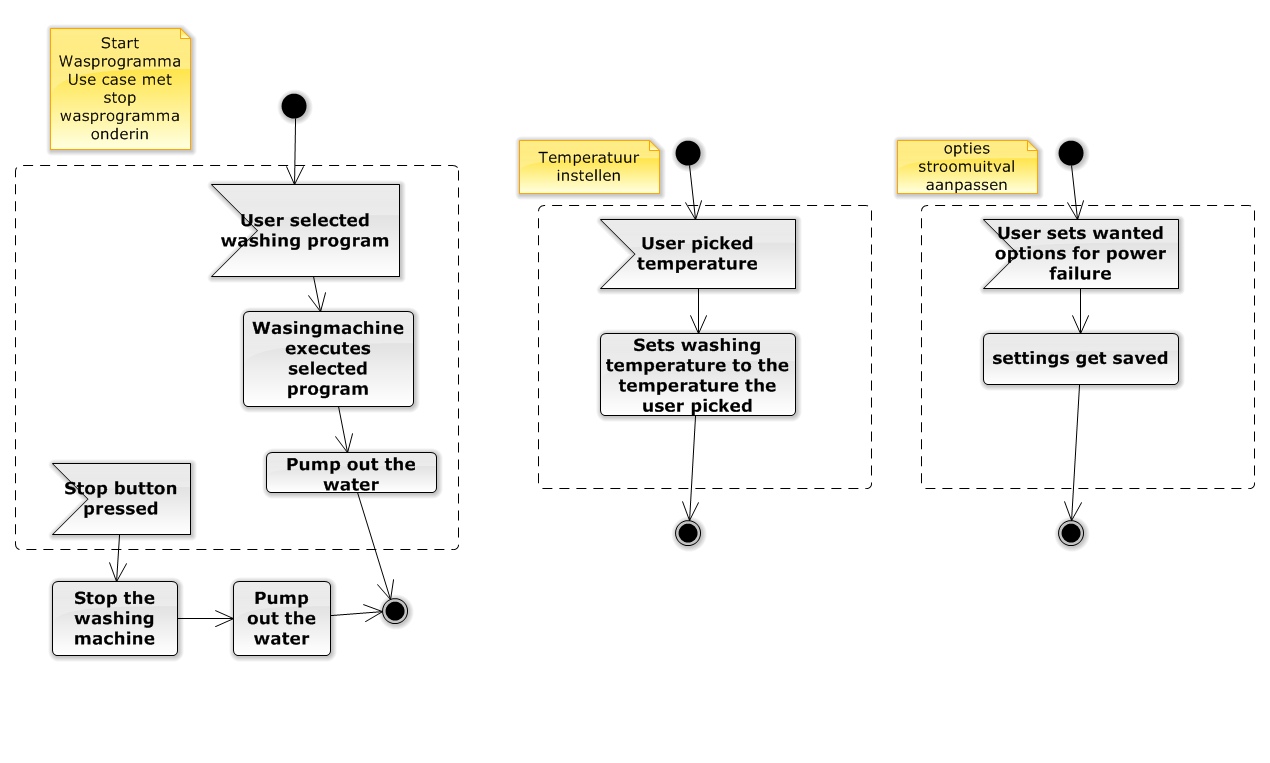
\includegraphics{activity_1.png}
}